

\documentclass{article}
\usepackage{pdfpages}
\usepackage{enumerate}
\usepackage[margin=1.4in, top=1in]{geometry}
\title{Teaching Statement}
\usepackage{mdframed}
\author{Joel Villatoro}
\date{}

\usepackage{blindtext}
\usepackage{hyperref}
\begin{document}
\vspace{-0.5in}
\maketitle

\section*{General Outlook} I find mathematics both fascinating and beautiful. I don't know about you but for me, when I encounter an interesting or beautiful fact in the world, my first instinct is to try to share it with someone else. My favorite part of teaching comes from helping students see the unexpected or counter-intuitive insights that make math so interesting.

Of course, students don't \emph{just} want to learn cool facts. They have specific objectives and they come to my classes with a variety of different backgrounds and experiences. Hence, my mission is always to provide a classroom environment that promotes both curiosity and enables each student to advance towards their goals.

\section*{Teaching Methodology}

Overall, I would describe my approach to teaching as one that emphasizes being pragmatic and empathetic. I like to focus on providing high quality instruction and to be responsive to the moment-to-moment needs of individual students. The specific techniques and practices I have experience with are ones that I would describe them as more or less standard practice for many US universities. That is, traditional lectures combined with a decent amount of active learning (in class and in discussion sections). However, I am not dogmatic by nature and I am quite open to experimenting with new approaches and ideas.

My past experiences teaching cover a wide range of ages, skill levels, backgrounds, and formats. I have taught in both the US and abroad. I believe that this has led me to becoming fairly skilled at adapting my teaching style to a wide variety of audiences. My students seem to agree. One of them told me in an email:
\begin{mdframed}
``Thank you, also I would like to note, you are a great professor, not every professor can deliver the information the way you can.'' - Calculus II Student (e-mail correspondence 2024)
\end{mdframed}
Although I am sure I can still improve. I do think clear and concise communication is one of my strengths as a lecturer.

During lectures, my style is to frequently prompt the students to suggest the next step. Time permitting, I like to ask them to try doing exercises themselves in class as well. My motivation for this is to try to maximize student engagement and to be able to get a feel for how students are receiving the material. I also like to employ geometric reasoning and visualizations to supplement my lectures. I encourage students to utilize graphic calculators and other tools to develop their intuition and guide calculations and I often demonstrate their use in class. 

As instructional aids, I create interactive visualization tools. For example, for my differential equations class I created a phase diagram visualization tool for linear ODEs\footnote{link: \url{https://www.desmos.com/calculator/tj3vn0rcqj}]}. Another little tool I'm proud of is a python notebook which illustrates a topological proof of the fundamental theorem of algebra \footnote{link:\url{https://colab.research.google.com/drive/1A898TEOGSHCNcYKM0BWP8YmsE2PLFz9M?usp=sharing}} which I created for another instructor. These tools have been well received by students. For example:
\begin{mdframed}
\textbf{Describe at least one activity (an exercise, project, assignment, etc.) in this course that helped you learn?} ``The use of graphing calculators like desmos'' - Differential Equations Course Feedback (2022)


\end{mdframed}

Historically I have placed a lot of emphasis on the value of discussion sections, homework, and group work. Although I am not a pedagogy researcher by training, I feel strongly that they are crucial (especially in larger classes) to developing deeper levels of understanding. I also really enjoy writing worksheets/recitation packets that provide a more interactive exploration of the material. For example, the following exercises from a differential equations worksheet:
\begin{mdframed}
\[    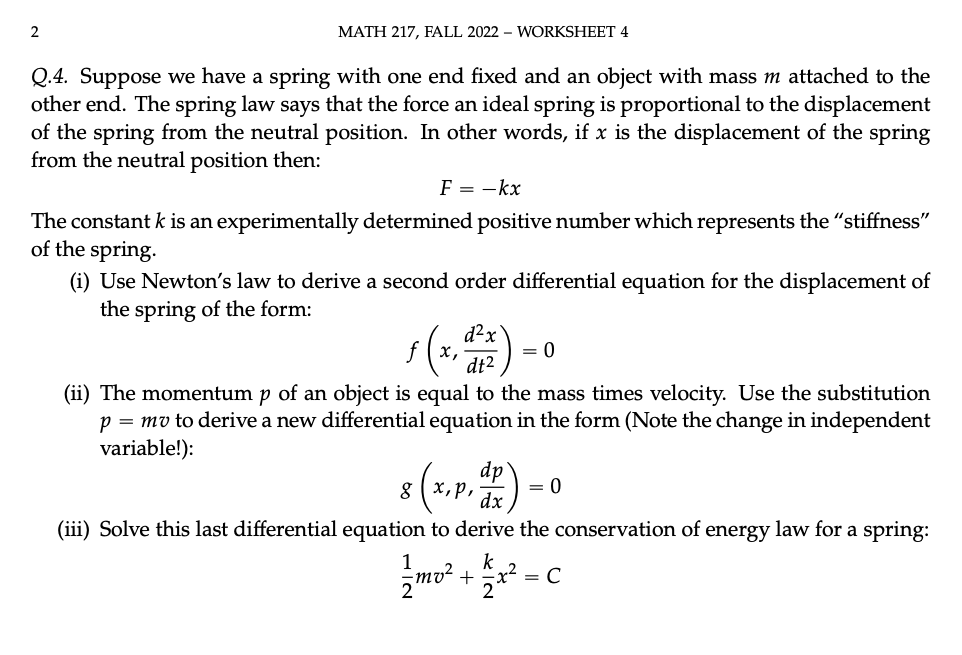
\includegraphics[width=5.5in]{example_exercise.png}\]
    \textbf{Remark}: The context for this exercise is that the students are studying how to transform differential equations using substitution methods. The goal of this exercises to show them ``real world'' application of these techniques.
\end{mdframed}
I've received positive feedback on this front as well. During my Fall 2022 Differential Equations Course many students praised the recitation packets as being a component of the course that contributed to their learning.


\section*{Mentorship}
In the past I have engaged in a variety of mentorship activities. 

At UIUC, I worked a mentor for undergraduates through the Illinois Geometry Lab. The Illinois Geometry Lab is a program run by the mathematics department which pairs small groups of undergraduates with a faculty member and graduate student. The faculty member provides the undergraduates with a project, usually a visualization of some mathematical concept, while the graduate student provides regular support while the undergraduates work on the project. I worked on multiple projects during my time but the first one involved numerical simulations of differential equations. At the time, I had little background in programming or computational mathematics. Despite this, I found that this was in many ways a benefit as I was better able to bond and connect with the undergraduate students by learning along side them. 

At KU Leuven my primary work as a mentor was supervising a Bachelor project. This involved advising a group of undergraduate mathematics majors while they studied chosen topic in mathematics. This experience was distinct from the IGL as the students were mathematics majors primarily interested in pursuing a career in pure mathematics. Much of our activities were reading and discussing mathematics articles and excerpts from textbooks. My primary role was to guide and advise them as they dipped their toe into reading and learning about topics in more advanced mathematics. The specific topic we investigated was cystallography and Bieberbach groups which was not a topic I was directly familiar with. Once again, I was reminded of how rewarding it can be to learn alongside my students.

\section*{Inclusive Teaching Practices}

I would describe my relationship to inclusiveness/diversity/equity as more personal than ideological. There were many moments in my career when I could have been turned away from mathematics if it were not for my mentors and role models who encouraged me to continue. From my point of view, it is a loss to our discipline any time a student is turned away from mathematics due to external factors like not feeling welcomed or a lack of support. Anyone interested in mathematics should feel as if they are invited to the party, so to speak.

To that end, I do my best to be sensitive to the needs and backgrounds of my students. Each student comes to college under unique circumstances that will inevitably shape their view of mathematics and their relationship to the subject. It seems clear to me that mathematics is not, overall, as diverse as it could be due a wide variety of social and cultural factors. People of many backgrounds often face serious challenges such as a lack of role models, implicit bias, and individual and systemic discrimination. 

One way I try to combat these issues is by promoting a ``growth mindset'' among my students. To elaborate, women and students from certain underrepresented groups sometimes struggle with an internalized ``fixed mindset'' which tells them that their ability to succeed in mathematics is intrinsic and unchangeable. Although all students can experience these feelings, I have found that they are particularly pernicious among students from underrepresented groups. For example, I have seen this frequently with the high school students I have interacted with through the Puertas program. Many of them, especially young Latina women, have sadly internalized a belief that they are simply ``not good at math'' and that this is an immutable characteristic. I find it important to confront this attitude head on and encourage students to instead adopt a growth mindset where they view mathematical ability as a skill that can be improved.

\end{document}
